%%%%%%%%%%%%%%%%%%%%% chapter.tex %%%%%%%%%%%%%%%%%%%%%%%%%%%%%%%%%
%
% sample chapter
%
% Use this file as a template for your own input.
%
%%%%%%%%%%%%%%%%%%%%%%%% Springer-Verlag %%%%%%%%%%%%%%%%%%%%%%%%%%
%\motto{Use the template \emph{chapter.tex} to style the various elements of your chapter content.}
\chapter{Chapter Heading}
\label{ascent} % Always give a unique label
% use \chaptermark{}
% to alter or adjust the chapter heading in the running head

\abstract*{
In situ coupling poses a unique set of challenges to the design of analysis and
visualization infrastructures.
%
When running with a simulation, resources, such as time and memory are constrained.
%
As simulation applications port to accelerator-based HPC architectures, so
must our analysis tools.
%
Further, integrating into a simulation's build system adds additional complexity
becomes difficult with more dependencies.
%
Our current community tools were not designed with these set of issues in mind.
%
Ascent is an emerging is situ analysis and visualization infrastructure that
addresses these challenges.
%
From Ascent's inception, we have targeted in situ use cases and many-core
architectures.
%
In this paper, we will discuss in detail Ascent's design considerations, data and control interfaces, system architecture, and success stories.
}

\section{The Ascent In Situ Infrastructure}
\label{ascent_overview}
Use the template \emph{chapter.tex} together with the document class SVMono (monograph-type books) or SVMult (edited books) to style the various elements of your chapter content conformable to the Springer Nature layout.

\section{Design Considerations}
\label{ascent_design_considerations}

\subsection{Reduce required dependencies and adhere to a lightweight memory footprint}
Software complexity. Ascent is less complex.

\subsection{Target exascale architectures: maximize constrained resources}
Ascent's primary in situ use case is tightly-coupled, i.e.,
Ascent shares the same computational resources (proximity) and
memory space as the simulaiton (access).
%
All core functionality in Ascent, transforming data
and making pictures, executes on the same hardware as the
simulation through portably performance abstractions such as
VTK-m and RAJA.
%
This enables Ascent to minimize data movement by directly accessing
the simulation data memory without making copies of the data.
%

Memory and time are both constrained resources in situ.

%
Simulations often consume almost all availble system memory,
leaving only a small fraction to in situ infrastructures.
%
It is imperative that Ascent uses memory as efficiently as possible
as not to exceed system memory.
%
To that end, Ascent can directly access simulation memory, whether it be
on the CPU or GPU.
%
While important, direct simulation memory access is only half
the battle of memory efficiency.
%
Visualization pipelines transforms data(e.g., isocontours) from
one form to another, and efficiently managing the memory consumed
by intermediate results is equally important.
%
\fix{possible example: contour of turbulence simulation on
structured grid can create a dataset larger than the original.}
%
In Ascent, we free memory used by intermediate results as soon
as they are not needed by downstream transforms.
%


%
Supercomper architectures have significanlty changed since
%
Current community visualization tools, such as ParaView and VisIt, were originally
designed to execute using one MPI rank per CPU core.
%

All core functionality(i.e., transforming data and making pictures) in
Ascent targets exascale architectures.

VTK-m, devil ray

\subsection{Provide simple and flexible data and control interfaces}

\subsection{Create tools to address in situ resource constraints , e.g., a flexible trigger system that allows users to express what is important}

\subsection{Simplify connection to other ecosystems, e.g., python, custom analysis, and Juptyer Notebooks}



\section{Data and Control Interfaces}
\label{ascent_data_control}
\subsection{Data Interface}
\subsubsection{Conduit: A foundation for in-memory data exchange}

\subsubsection{Mesh Blueprint: An in-memory mesh description interface co-designed with simulation applications
System Architecture}

\subsection{DataObject}

I feel like we should list the different data models we currenlty support and how we
move from one to the other.

\subsection{Control Interface}

\subsubsection{Ascent Actions: A declarative interface supporting multiple programing languages and file-based user control}

\subsubsection{Core user-facing concepts: Scenes, Transforms, Extracts, Queries, and Triggers}


\section{System Architecture}
\label{ascent_architecture}
In the previous section, we described Ascent's high-level abstractions and
capabilities.
%
This section discusses Ascent's system architecture starting at its inner layer, Flow,
and moving outward.

\subsection{Flow: A data-type agnostic data-flow based architecture}
\label{sec:flow}
Ascent uses a graph-based data-flow architecture.
The data-flow architecture allows Ascent to track, re-use, and cleanup intermediate
results efficiently while implementing complex visualization pipelines.
The design also abstracts how we register and execute operations,
which simplifies adding new features.

At Ascent's core is a simple data-flow library known as Flow, that
composes and executes filters, which are the basic unit of execution in Ascent.
%
Flow is an evolution of a Python data-flow network
~\cite{flow_reference}, but unlike its ancestor, Flow is a C++
library.
%
Flow supports composing and executing directed acyclic graphs
(DAGs) composed of filters~\cite{LarsenAscent}.

There are four components to Flow:
\begin{itemize}
  \item \textbf{Filter}: basic unit of execution.
  \item \textbf{Graph}: contains the filter graph and manages the adding of
filters.
  \item \textbf{Registry}: manages the lifetime of filter results.
  \item \textbf{Workspace}: contains both the registry and filter graph,
coordinates graph execution.
\end{itemize}

\paragraph{Flow Filters}
Flow filters are the basic unit of execution inside of Ascent, and
almost all functionality inside of Ascent is implemented as a Flow filter.
%
Adding new capabilities to Ascent means wrapping that functionality inside
a flow filter.
%
Filters declare an interface, i.e., how many inputs a filter has and
if there is an output, and filters are passed a set of parameters inside
of a Conduit node (see \S\ref{Conduit}).
%
Filter inputs are tracked as arbitrary pointers and runtime features allow
filters to identify and obtain concrete types for processing.
%
In terms of Ascent actions, pipeline filters become part of a chain of
data transformations and would minimally have an input
data set and an output data set, while scenes and extracts
become sinks that have an input data set and no output.
%

\paragraph{Graph}
The graph is a series of Flow filters connected together into
a DAG.
%
The graph is responsible for storing filters and connections
between filters.
%
The primary graph interface supports adding filters and connecting
filter ports (e.g., inputs and outputs) together.

\paragraph{Registry}
The registry is a key-value data store used to manage the intermediate
results of filters inside the data-flow network.
%
Keys within the registry are reference counted, and data contained
inside the registry is deleted when the reference counts reach zero.
%
While the data associated with a key can be a pointer to any type,
the majority of the data stored in the registry are Conduit Nodes
or VTK-m data sets.


\paragraph{Workspace}
The workspace is a container for both the graph and the registry,
and the workspace is responsible for executing the DAG.
%
Additionally, the workspace manages the lists of known filters.
%
A filter must be registered with the workspace in order to be added to the
graph, and once registered, a filter can be added to the graph by name.
%
Flow uses a topological sort to ensure proper filter execution order,
to track all intermediate results, and to provide basic memory management capabilities.
During execution, the workspace provides the registry with reference counts that reflect graph connections, allowing intermediate results to be efficiently managed.

%
Multiple workspaces can co-exist, and in fact, Ascent uses a separate Flow workspace
to evaluate expressions within the Ascent runtime.
%

\subsection{Runtime}
The Ascent runtime builds on top of Flow, and the main responsibility of the
runtime is to translate user actions into data-flow networks.
%
For example, when a user describes a series of data transformations inside of a pipeline,
the runtime adds the corresponding filter for each transformation to
the internal Flow graph.
%
Some actions, like the contour filter, have exactly one filter that the runtime
adds when translating actions, while other actions add more than one filter to the graph.
%
Fig.~\ref{img:flow_graph} shows a simplified view of a data-flow network constructed by the
runtime to create contours of a simulation field and rendering an image of the result.
%

\begin{figure}
\centering
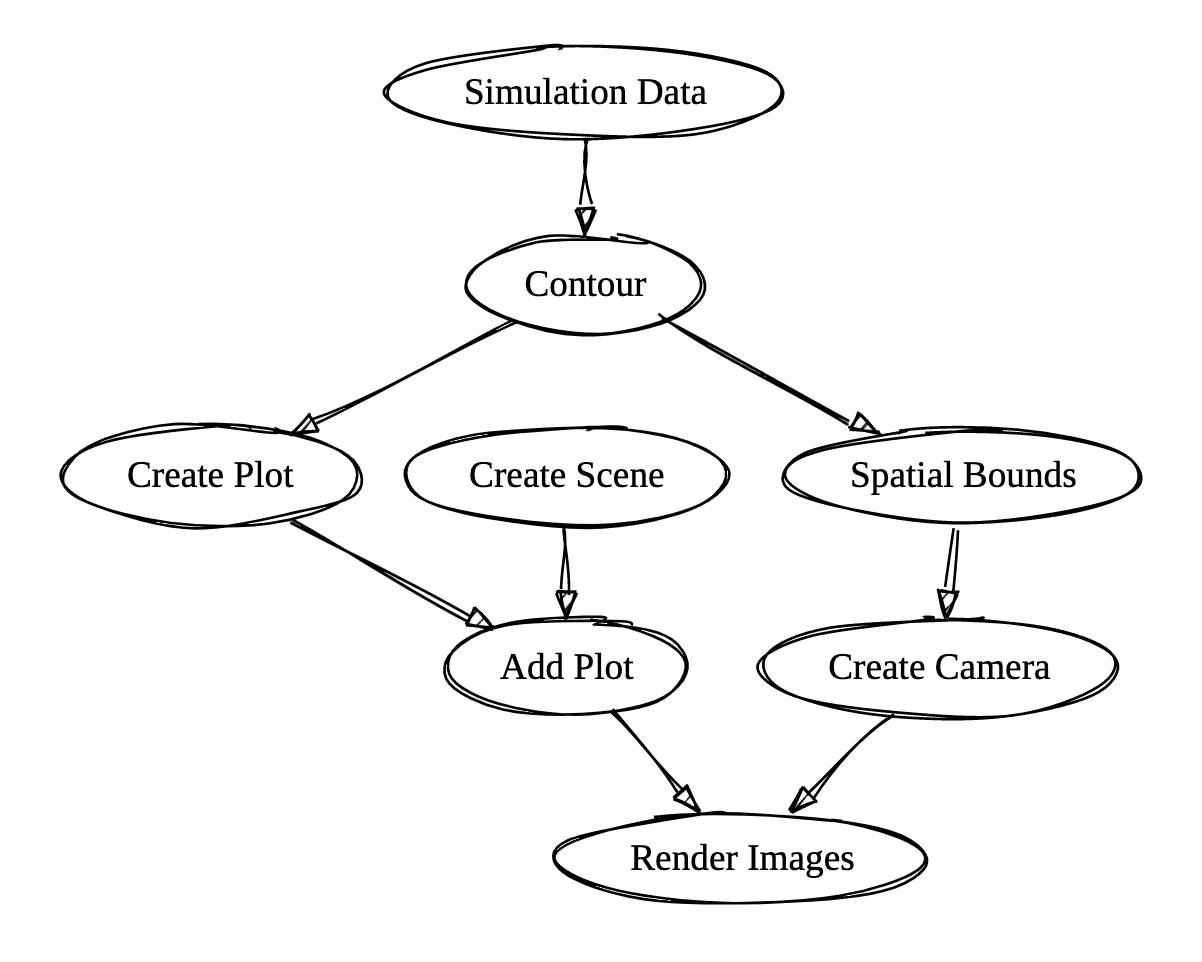
\includegraphics[width=0.6\textwidth]{images/flow_graph}
\caption{\label{img:flow_graph} An example data flow network using Flow assembled by the Ascent runtime.}
\end{figure}

Internally, the runtime maintains a list of registered filters to map
user-facing API names to the corresponding Flow filters which are hidden
from the user.
%
In addition to mapping API calls to Flow filters, the filter map also specifies
in what actions a filter can be used.
%
Runtime Filters can be registered as either a ``transform'' or an ``extract.''
%
Transforms are only callable inside of pipelines and extracts can only be called at the end of a pipeline.
%
Built-in functionality is registered internally with the Ascent runtime when Ascent is initialized.


The runtime also exposes the filter registration of the underlying data flow network which
allows the runtime to inherit Flow's flexibility.
%
Simulations, or other analysis libraries, are free to register custom capability at
runtime, and this allows outside functionality to build off the capability
provided by Ascent.
%
Just like internal filters, custom filters can either be registered as transforms or extracts,
and can directly connect with simulation data or consume the results of a pipeline.
%

The other responsibility of the runtime is to interface with the simulation through Ascent's
main API calls.
%
The runtime consumes configuration options like MPI communicators, exception
handling, and what
backends (e.g., OpenMP or CUDA) to execute code on.
%
Additionally, the simulation's mesh data and the actions are all passed to the runtime.

\subsubsection{Parallelism in Ascent}
Ascent is a hybrid-parallel library, meaning that it uses both
distributed-memory (e.g., MPI) and shared-memory parallelism
(e.g., CUDA and OpenMP), and Ascent is primarily
tightly-coupled with simulations.
%
In the tightly-coupled paradigm, simulations control how parallelism is used, so
it is imperative that Ascent's functionality be capable of running
on the same architectures using the same types of parallelism as the
simulations.
%
Ascent supports many different parallel configurations including
one MPI rank per core (i.e., no shared-memory parallelism), one rank
per GPU, and one rank per node.
%
While Ascent does internally leverage shared-memory parallelism
for expressions, the majority of the shared-memory parallelism comes
from Ascent's components such as VTK-m and Devil Ray.

\paragraph{Distributed-Memory Parallelism}
Within Ascent, all MPI ranks receive the same set of actions.
%
Since the actions are the same, all MPI ranks create and execute the same graph,
meaning that all flow filters execute on all ranks.
%
Ascent guarantees that each filter is given full control of MPI communication,
and filters are free to use MPI anyway they see fit, including
creating asynchronous tasks.
%
Some filters, such as threshold, do not need to use any
MPI communication, i.e., each block of data is processed independently,
but other filters, such as particle advection, use MPI to pass particles
from one rank to another.
%
For mesh data, as discussed in \S\ref{ascent_control},
each MPI rank receives data published by the simulation, and
Ascent does not redistribute the data.
%
That said, filters can change the data distribution (e.g., resampling
an unstructured grid onto a uniform grid), although this can be a costly
operation.
%

\paragraph{Shared-Memory Parallelism}
Ascent's main components use portable performance abstraction layers to
take advantage of the different types of shared-memory parallelism on
modern supercomputers.
%
For example, VTK-m is itself a portable performance layer designed specifically
for visualization and currently supports OpenMP, CUDA, and TBB.
%
Devil Ray, while not itself a portable performance layer, uses RAJA to execute
on different architectures, supporting OpenMP, CUDA, HIP, and TBB.

\subsubsection{Data Set Representations}
Ascent uses an internal data abstraction, called the data object, as the input
and outputs of filters.
%
The data object is responsible for transforming data from one in-memory format
to another without unnecessary copies.
%
By using this abstraction, filters can ask for whatever data set
representation they need, however, the conversions between data
representations are not always one-to-one and may not always
result in a shallow copy.
%

To support multiple data set representations, there must be a common
set of supported features, but not all data models Ascent uses
support the same set of features.
%
Since Ascent uses Blueprint(see \S\ref{Blueprint}) as its data interface to simulations,
all other data models must sometimes be adapted to support additional
features.
%
For example, Blueprint supports multiple topologies in the same data set
but VTK-m only supports a single topology.
%
To handle this correctly within Ascent, we wrap the data sets in a container
that treats each topology as individual VTK-m data sets.
%


\section{Success Stories}
\label{ascent_success}

%%%%%%%%%%%%%%%%%%%%%%%% referenc.tex %%%%%%%%%%%%%%%%%%%%%%%%%%%%%%
% sample references
% %
% Use this file as a template for your own input.
%
%%%%%%%%%%%%%%%%%%%%%%%% Springer-Verlag %%%%%%%%%%%%%%%%%%%%%%%%%%
%
% BibTeX users please use
% \bibliographystyle{}
% \bibliography{}
%
\biblstarthook{References may be \textit{cited} in the text either by number (preferred) or by author/year.\footnote{Make sure that all references from the list are cited in the text. Those not cited should be moved to a separate \textit{Further Reading} section or chapter.} If the citatiion in the text is numbered, the reference list should be arranged in ascending order. If the citation in the text is author/year, the reference list should be \textit{sorted} alphabetically and if there are several works by the same author, the following order should be used:
\begin{enumerate}
\item all works by the author alone, ordered chronologically by year of publication
\item all works by the author with a coauthor, ordered alphabetically by coauthor
\item all works by the author with several coauthors, ordered chronologically by year of publication.
\end{enumerate}
The \textit{styling} of references\footnote{Always use the standard abbreviation of a journal's name according to the ISSN \textit{List of Title Word Abbreviations}, see \url{http://www.issn.org/en/node/344}} depends on the subject of your book:
\begin{itemize}
\item The \textit{two} recommended styles for references in books on \textit{mathematical, physical, statistical and computer sciences} are depicted in ~\cite{science-contrib, science-online, science-mono, science-journal, science-DOI} and ~\cite{phys-online, phys-mono, phys-journal, phys-DOI, phys-contrib}.
\item Examples of the most commonly used reference style in books on \textit{Psychology, Social Sciences} are~\cite{psysoc-mono, psysoc-online,psysoc-journal, psysoc-contrib, psysoc-DOI}.
\item Examples for references in books on \textit{Humanities, Linguistics, Philosophy} are~\cite{humlinphil-journal, humlinphil-contrib, humlinphil-mono, humlinphil-online, humlinphil-DOI}.
\item Examples of the basic Springer Nature style used in publications on a wide range of subjects such as \textit{Computer Science, Economics, Engineering, Geosciences, Life Sciences, Medicine, Biomedicine} are ~\cite{basic-contrib, basic-online, basic-journal, basic-DOI, basic-mono}. 
\end{itemize}
}

\begin{thebibliography}{99.}%
% and use \bibitem to create references.
%
% Use the following syntax and markup for your references if 
% the subject of your book is from the field 
% "Mathematics, Physics, Statistics, Computer Science"
%
% Contribution 
\bibitem{science-contrib} Broy, M.: Software engineering --- from auxiliary to key technologies. In: Broy, M., Dener, E. (eds.) Software Pioneers, pp. 10-13. Springer, Heidelberg (2002)
%
% Online Document
\bibitem{science-online} Dod, J.: Effective substances. In: The Dictionary of Substances and Their Effects. Royal Society of Chemistry (1999) Available via DIALOG. \\
\url{http://www.rsc.org/dose/title of subordinate document. Cited 15 Jan 1999}
%
% Monograph
\bibitem{science-mono} Geddes, K.O., Czapor, S.R., Labahn, G.: Algorithms for Computer Algebra. Kluwer, Boston (1992) 
%
% Journal article
\bibitem{science-journal} Hamburger, C.: Quasimonotonicity, regularity and duality for nonlinear systems of partial differential equations. Ann. Mat. Pura. Appl. \textbf{169}, 321--354 (1995)
%
% Journal article by DOI
\bibitem{science-DOI} Slifka, M.K., Whitton, J.L.: Clinical implications of dysregulated cytokine production. J. Mol. Med. (2000) doi: 10.1007/s001090000086 
%
\bigskip

% Use the following (APS) syntax and markup for your references if 
% the subject of your book is from the field 
% "Mathematics, Physics, Statistics, Computer Science"
%
% Online Document
\bibitem{phys-online} J. Dod, in \textit{The Dictionary of Substances and Their Effects}, Royal Society of Chemistry. (Available via DIALOG, 1999), 
\url{http://www.rsc.org/dose/title of subordinate document. Cited 15 Jan 1999}
%
% Monograph
\bibitem{phys-mono} H. Ibach, H. L\"uth, \textit{Solid-State Physics}, 2nd edn. (Springer, New York, 1996), pp. 45-56 
%
% Journal article
\bibitem{phys-journal} S. Preuss, A. Demchuk Jr., M. Stuke, Appl. Phys. A \textbf{61}
%
% Journal article by DOI
\bibitem{phys-DOI} M.K. Slifka, J.L. Whitton, J. Mol. Med., doi: 10.1007/s001090000086
%
% Contribution 
\bibitem{phys-contrib} S.E. Smith, in \textit{Neuromuscular Junction}, ed. by E. Zaimis. Handbook of Experimental Pharmacology, vol 42 (Springer, Heidelberg, 1976), p. 593
%
\bigskip
%
% Use the following syntax and markup for your references if 
% the subject of your book is from the field 
% "Psychology, Social Sciences"
%
%
% Monograph
\bibitem{psysoc-mono} Calfee, R.~C., \& Valencia, R.~R. (1991). \textit{APA guide to preparing manuscripts for journal publication.} Washington, DC: American Psychological Association.
%
% Online Document
\bibitem{psysoc-online} Dod, J. (1999). Effective substances. In: The dictionary of substances and their effects. Royal Society of Chemistry. Available via DIALOG. \\
\url{http://www.rsc.org/dose/Effective substances.} Cited 15 Jan 1999.
%
% Journal article
\bibitem{psysoc-journal} Harris, M., Karper, E., Stacks, G., Hoffman, D., DeNiro, R., Cruz, P., et al. (2001). Writing labs and the Hollywood connection. \textit{J Film} Writing, 44(3), 213--245.
%
% Contribution 
\bibitem{psysoc-contrib} O'Neil, J.~M., \& Egan, J. (1992). Men's and women's gender role journeys: Metaphor for healing, transition, and transformation. In B.~R. Wainrig (Ed.), \textit{Gender issues across the life cycle} (pp. 107--123). New York: Springer.
%
% Journal article by DOI
\bibitem{psysoc-DOI}Kreger, M., Brindis, C.D., Manuel, D.M., Sassoubre, L. (2007). Lessons learned in systems change initiatives: benchmarks and indicators. \textit{American Journal of Community Psychology}, doi: 10.1007/s10464-007-9108-14.
%
%
% Use the following syntax and markup for your references if 
% the subject of your book is from the field 
% "Humanities, Linguistics, Philosophy"
%
\bigskip
%
% Journal article
\bibitem{humlinphil-journal} Alber John, Daniel C. O'Connell, and Sabine Kowal. 2002. Personal perspective in TV interviews. \textit{Pragmatics} 12:257--271
%
% Contribution 
\bibitem{humlinphil-contrib} Cameron, Deborah. 1997. Theoretical debates in feminist linguistics: Questions of sex and gender. In \textit{Gender and discourse}, ed. Ruth Wodak, 99--119. London: Sage Publications.
%
% Monograph
\bibitem{humlinphil-mono} Cameron, Deborah. 1985. \textit{Feminism and linguistic theory.} New York: St. Martin's Press.
%
% Online Document
\bibitem{humlinphil-online} Dod, Jake. 1999. Effective substances. In: The dictionary of substances and their effects. Royal Society of Chemistry. Available via DIALOG. \\
http://www.rsc.org/dose/title of subordinate document. Cited 15 Jan 1999
%
% Journal article by DOI
\bibitem{humlinphil-DOI} Suleiman, Camelia, Daniel C. O'Connell, and Sabine Kowal. 2002. `If you and I, if we, in this later day, lose that sacred fire...': Perspective in political interviews. \textit{Journal of Psycholinguistic Research}. doi: 10.1023/A:1015592129296.
%
%
%
\bigskip
%
%
% Use the following syntax and markup for your references if 
% the subject of your book is from the field 
% "Computer Science, Economics, Engineering, Geosciences, Life Sciences"
%
%
% Contribution 
\bibitem{basic-contrib} Brown B, Aaron M (2001) The politics of nature. In: Smith J (ed) The rise of modern genomics, 3rd edn. Wiley, New York 
%
% Online Document
\bibitem{basic-online} Dod J (1999) Effective Substances. In: The dictionary of substances and their effects. Royal Society of Chemistry. Available via DIALOG. \\
\url{http://www.rsc.org/dose/title of subordinate document. Cited 15 Jan 1999}
%
% Journal article by DOI
\bibitem{basic-DOI} Slifka MK, Whitton JL (2000) Clinical implications of dysregulated cytokine production. J Mol Med, doi: 10.1007/s001090000086
%
% Journal article
\bibitem{basic-journal} Smith J, Jones M Jr, Houghton L et al (1999) Future of health insurance. N Engl J Med 965:325--329
%
% Monograph
\bibitem{basic-mono} South J, Blass B (2001) The future of modern genomics. Blackwell, London 
%
\end{thebibliography}

